\documentclass{article}
\usepackage{longtable} % 支持长表格
\usepackage{verbatim}  % 支持代码
\usepackage{geometry}  % 控制页面布局
\geometry{a4paper, margin=1in}
\usepackage{amsmath}
\usepackage{graphicx}
\usepackage{listings}
\usepackage{pythonhighlight}
\usepackage[UTF8]{ctex}


\title{第四次作业}
\author{时伟杰}
\date{\today}
\begin{document}

\maketitle

\section{相关介绍}
调试与性能分析:如何高效调试代码并进行性能优化。通过工具如 gdb(GNU调试器)、valgrind(内存调试和分析工具)和 strace(系统调用跟踪器)等,开发者可以找到代码中的问题并提升运行效率。文章还讨论了如何使用性能分析工具检测瓶颈,帮助减少资源消耗。
元编程:元编程涉及编写可以生成或修改其他代码的程序。文章介绍了宏和模板的使用,通过元编程减少代码冗余,提高开发效率。尤其在复杂的系统设计中,元编程有助于抽象和自动化重复任务。
杂项工具:本篇涵盖了工作流中的一些重要工具和技巧,包括如何加强系统的安全性,编写自动化脚本,优化命令行操作。它还介绍了一些提高生产力的程序,帮助开发者更好地管理时间和资源。这个部分提供了多种提升个人工作流的建议。
pytorch:PyTorch是一个开源的深度学习框架,由Facebook开发,广泛用于研究和生产环境。它提供了灵活的动态计算图结构,使用户能够轻松实现各种神经网络模型。PyTorch主要使用Python编写,并支持GPU加速。其核心组件包括张量计算、自动求导(autograd)和神经网络模块(torch.nn)。PyTorch的易用性和灵活性使其非常适合快速原型设计和复杂模型的研究,广泛用于计算机视觉、自然语言处理等领域。
\section{实例演示}

\noindent
\begin{longtable}{|c|p{10cm}|l|}
\hline
\textbf{编号} & \textbf{代码实例} & \textbf{解释} \\
\hline
1 & \verb|gdb ./a.out| & 启动GNU调试器调试可执行文件 \\
\hline
2 & \verb|break main| & 在main函数处设置断点,程序将在此处暂停执行 \\
\hline
3 & \verb|step| & 一步步执行代码,查看变量和状态 \\
\hline
4 & \verb|print var| & 查看当前作用域中变量var的值 \\
\hline
5 & \verb|continue| & 让程序继续执行直到下一个断点或结束 \\
\hline
6 & \verb|valgrind --leak-check=full ./a.out| & 检查程序中是否存在内存泄漏 \\
\hline
7 & \verb|strace ./a.out| & 跟踪程序执行过程中所有系统调用 \\
\hline
8 & \verb|perf stat ./a.out| & 显示程序的CPU使用统计信息 \\
\hline
9 & \verb|strace -e open ./a.out| & 仅跟踪文件打开的系统调用 \\
\hline
10 & \verb|gprof ./a.out gmon.out| & 分析函数的调用频率和消耗的时间 \\
\hline
11 & \verb|top| & 监控系统中各个进程的CPU和内存利用情况 \\
\hline
12 & \verb|valgrind --tool=massif ./a.out| & 分析程序内存使用情况的详细信息 \\
\hline
13 & \verb|backtrace| & 在gdb中显示当前函数调用栈,定位问题函数 \\
\hline
14 & \verb|valgrind --tool=memcheck ./a.out| & 查找程序中的内存访问错误 \\
\hline
15 & \verb|time ./a.out| & 显示程序的执行时间,包括用户态和系统态时间 \\
\hline
16 & \verb|htop| & 提供类似top的更直观的进程监控界面 \\
\hline
17 & \verb|strace -f ./a.out| & 跟踪多线程程序中的系统调用 \\
\hline
18 & \verb|finish| & 在gdb中执行到当前函数返回,观察其返回值 \\
\hline
19 & \verb|perf record ./a.out| \newline \verb|perf report| & 记录程序性能并生成报告 \\
\hline
20 & \verb|memusage ./a.out| & 捕获程序的内存分配情况,适用于追踪大规模内存使用问题 \\
\hline
21 & \verb|#define PI 3.14| & 定义一个名为PI的常量 \\
\hline
22 & \verb|exec("print('Hello')")| & 通过exec执行代码字符串 \\
\hline
23 & \verb|all: gcc main.c -o main| & 使用Makefile自动编译C程序 \\
\hline
24 & \verb|#ifdef DEBUG| & 根据条件编译代码 \\
\hline
25 & \verb|def hello(): pass| & 定义一个空函数 \\
\hline
26 & \verb|(defmacro when (cond &body body) ...)| & 创建when宏,简化if逻辑 \\
\hline
27 & \verb|class Meta(type): pass| & 使用元类控制类创建流程 \\
\hline
28 & \verb|test: pytest tests/| & 定义测试规则以运行pytest \\
\hline
29 & \verb|template <typename T> T add(T a, T b) { return a + b; }| & 使用模板实现泛型加法 \\
\hline
30 & \verb|for file in *.txt; do mv "$file" "${file%.txt}.md"; done| & 遍历目录中所有.txt文件并重命名为.md文件 \\
\hline
31 & \verb|history | grep 'git'| & 通过grep在命令历史中搜索包含“git”的命令 \\
\hline
32 & \verb|git bisect start| \newline \verb|git bisect bad HEAD| \newline \verb|git bisect good <commit-hash>| & 使用Git二分查找Bug \\
\hline
33 & \verb|tmux new -s my_session| & 创建一个名为my_session的tmux会话 \\
\hline
34 & \verb|awk -F"," '{sum += $2} END {print sum}' data.csv| & 使用awk计算CSV文件中第二列的总和 \\
\hline
35 & \verb|ssh-keygen -t rsa -b 4096| \newline \verb|ssh-copy-id user@server.com| & 生成RSA SSH密钥并将其复制到服务器 \\
\hline
36 & \verb|rename 's/\.jpg$/\.png/' *.jpg| & 批量将当前目录中的.jpg文件扩展名修改为.png \\
\hline
37 & \verb|python3 -m http.server 8080| & 启动简易HTTP服务器,监听8080端口 \\
\hline
38 & \verb|fd 'myfile'| & 使用fd命令快速查找文件 \\
\hline
39 & \verb|git stash push -m "work-in-progress"| \newline \verb|git stash apply| & git stash将更改暂存并恢复 \\
\hline
40 & \verb|import torch| \newline \verb|x = torch.Tensor([[1, 2], [3, 4]])| \newline \verb|print(x)| & 创建并打印一个2x2的浮点型张量 \\
\hline
41 & \verb|y = torch.Tensor([[5, 6], [7, 8]])| \newline \verb|result = x + y| \newline \verb|print(result)| & 进行两个张量的加法运算 \\
\hline
42 & \verb|model = torch.nn.Linear(1, 1)| \newline \verb|inputs = torch.tensor([[1.0], [2.0], [3.0]])| \newline \verb|outputs = model(inputs)| \newline \verb|print(outputs)| & 构建一个简单的线性回归模型并进行前向传播 \\
\hline
43 & \verb|class CNN(torch.nn.Module):| \newline \verb|def __init__(self):| \newline \verb|super(CNN, self).__init__()| \newline \verb|self.conv1 = torch.nn.Conv2d(1, 16, 3)| \newline \verb|def forward(self, x):| \newline \verb|return self.conv1(x)| & 构建一个简单的CNN模型 \\
\hline

\end{longtable}
\section{截图示例}

\begin{figure}[htbp]
\centering
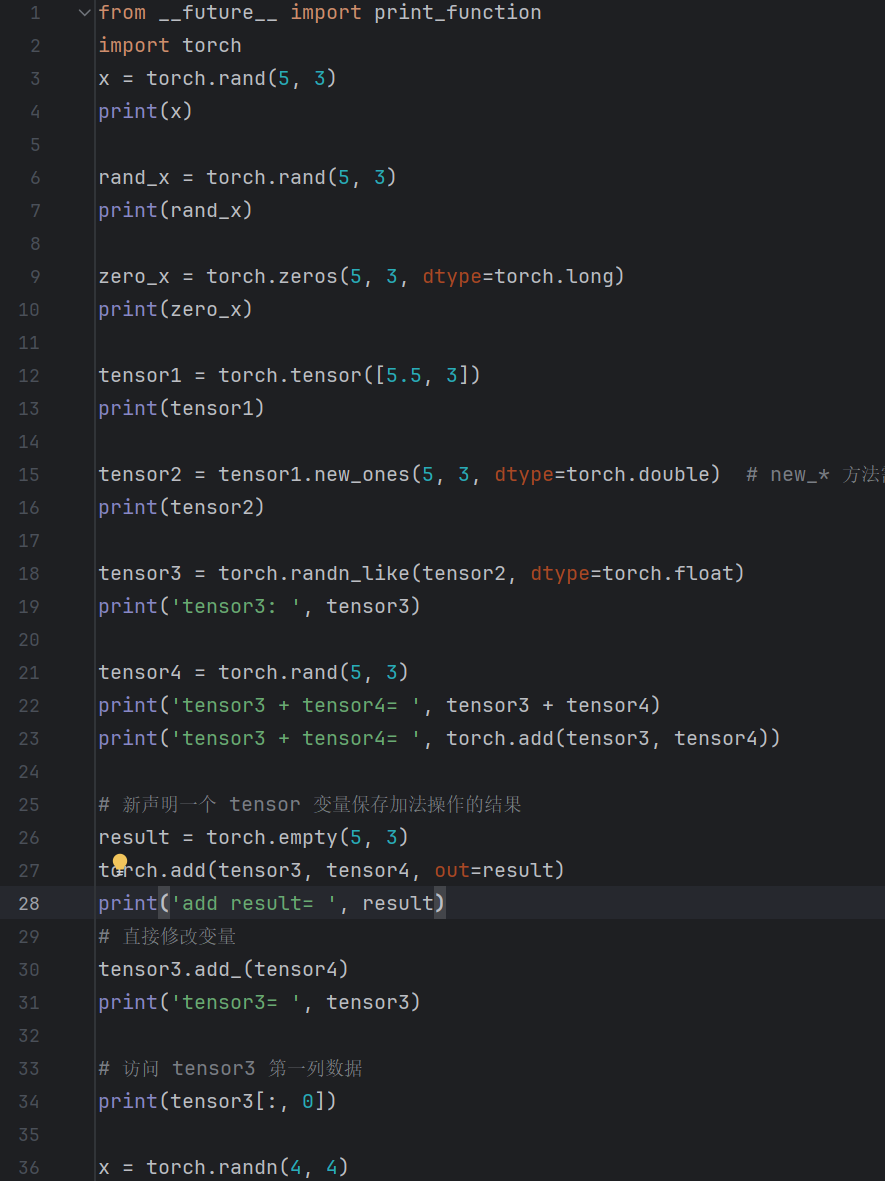
\includegraphics[width=0.7\textwidth]{1.png}
\caption{代码}
\end{figure}

\begin{figure}[htbp]
\centering
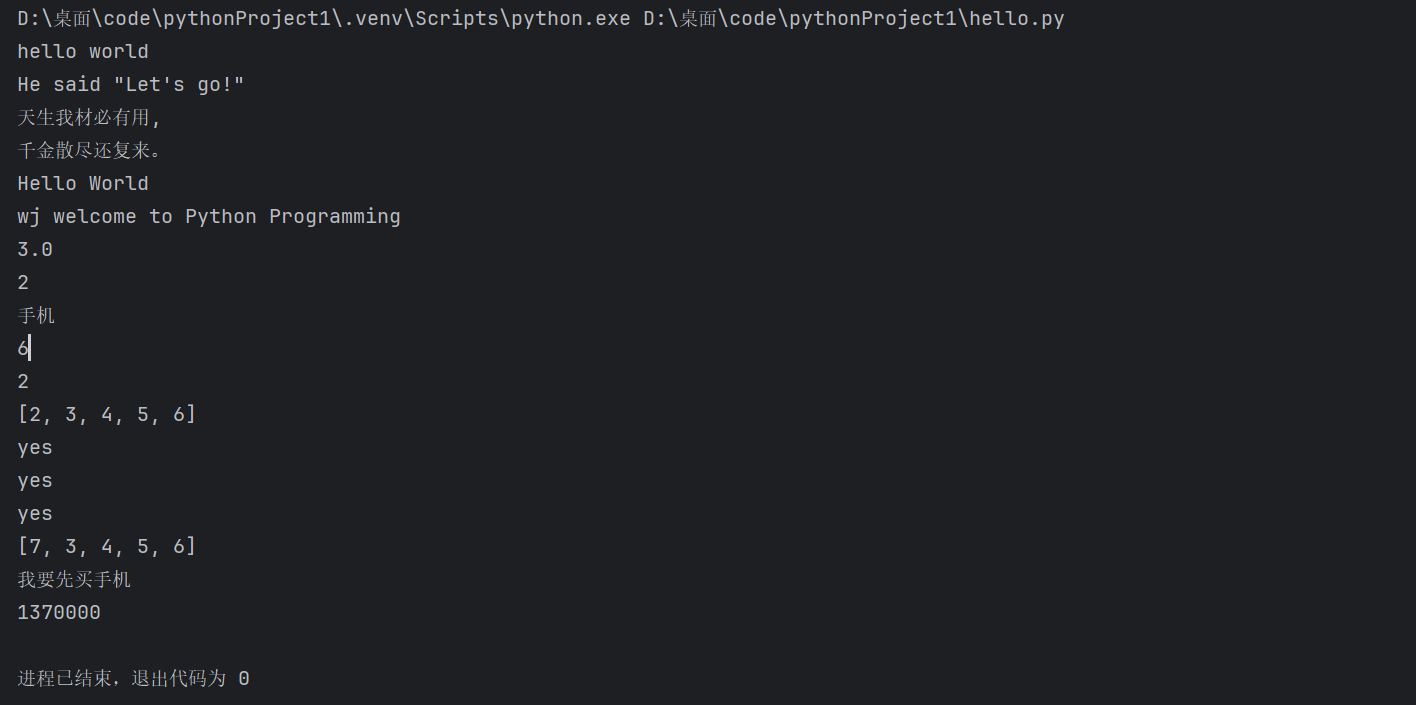
\includegraphics[width=0.8\textwidth]{2.png}
\caption{代码}
\end{figure}

\begin{figure}[htbp]
\centering
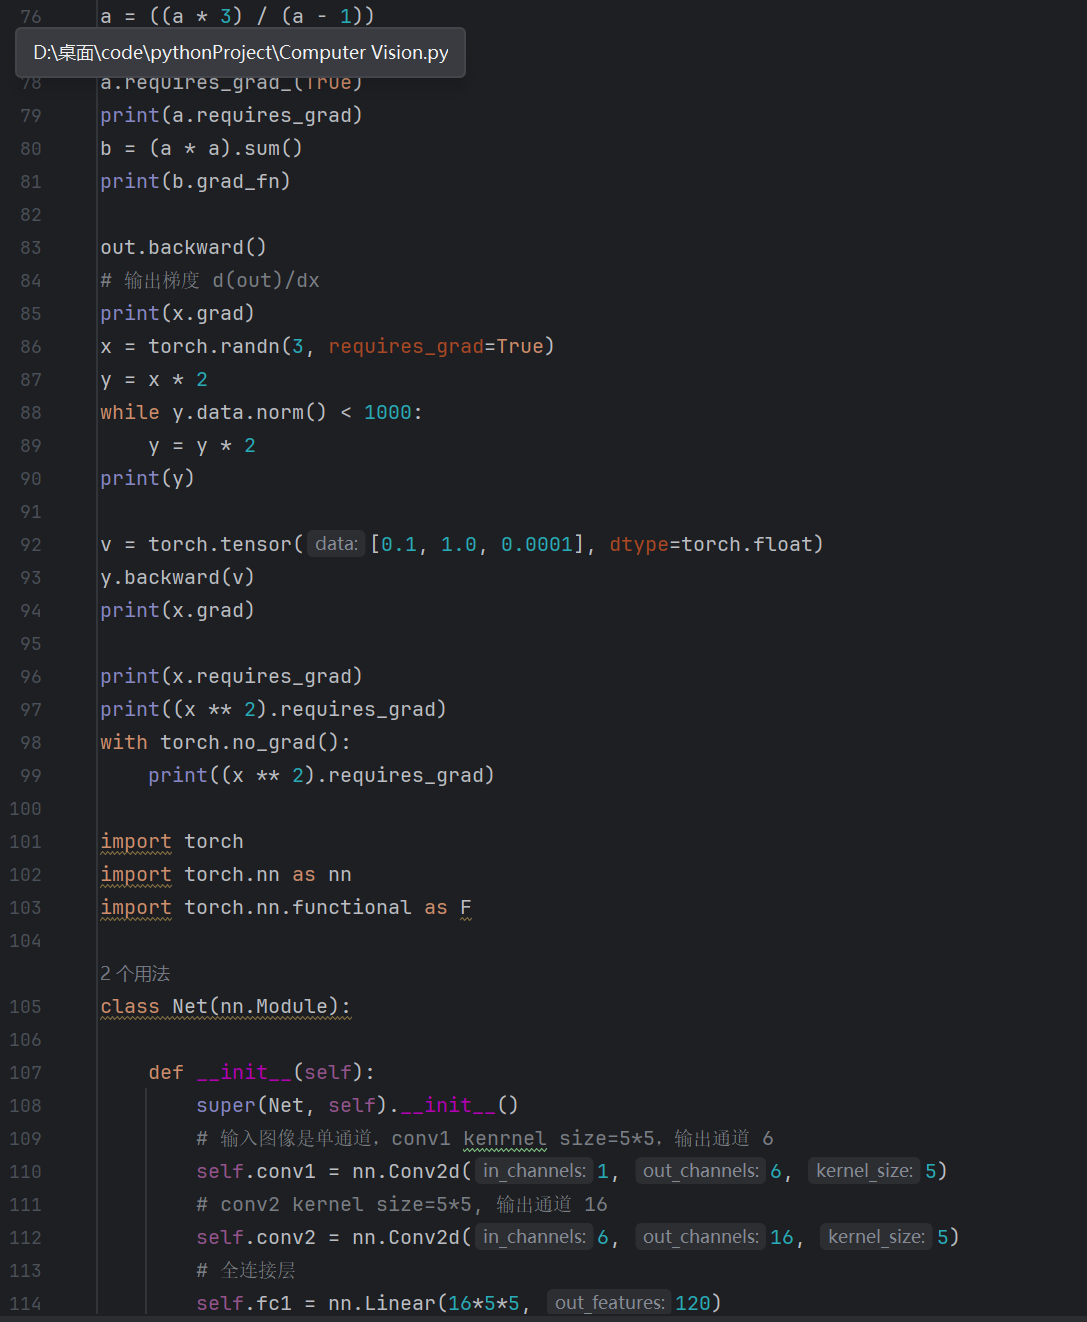
\includegraphics[width=0.8\textwidth]{3.png}
\caption{代码}
\end{figure}

\begin{figure}[htbp]
\centering
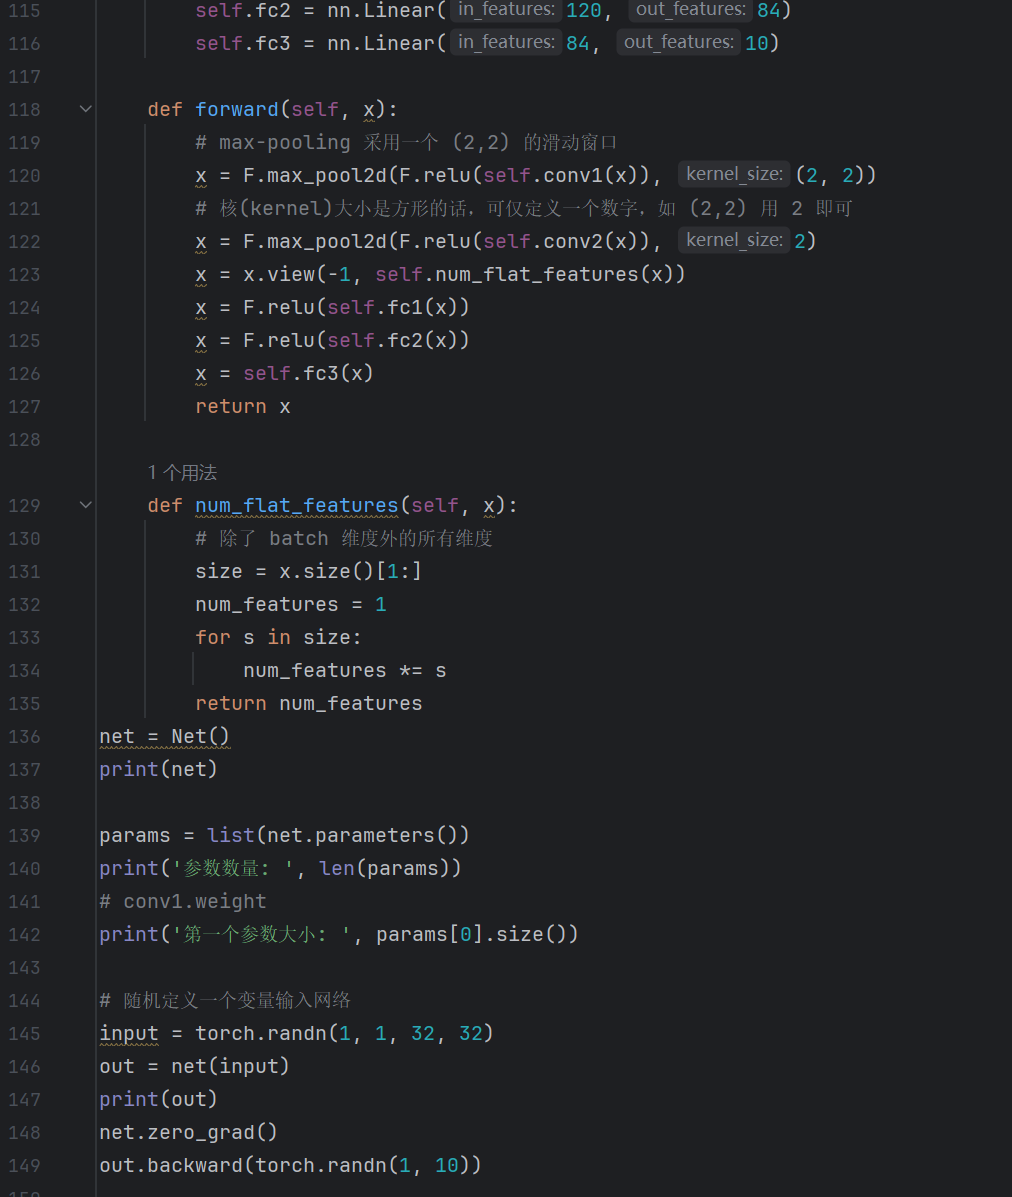
\includegraphics[width=0.8\textwidth]{4.png}
\caption{代码}
\end{figure}

\begin{figure}[htbp]
\centering
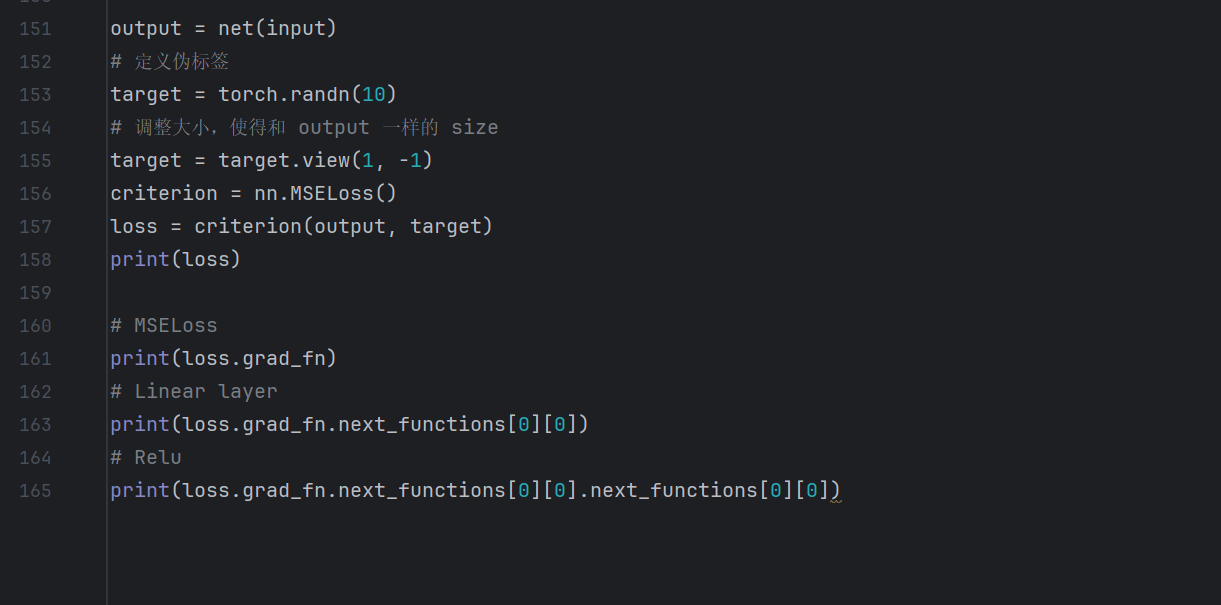
\includegraphics[width=0.7\textwidth]{5.png}
\caption{代码}
\end{figure}

\begin{figure}[htbp]
\centering
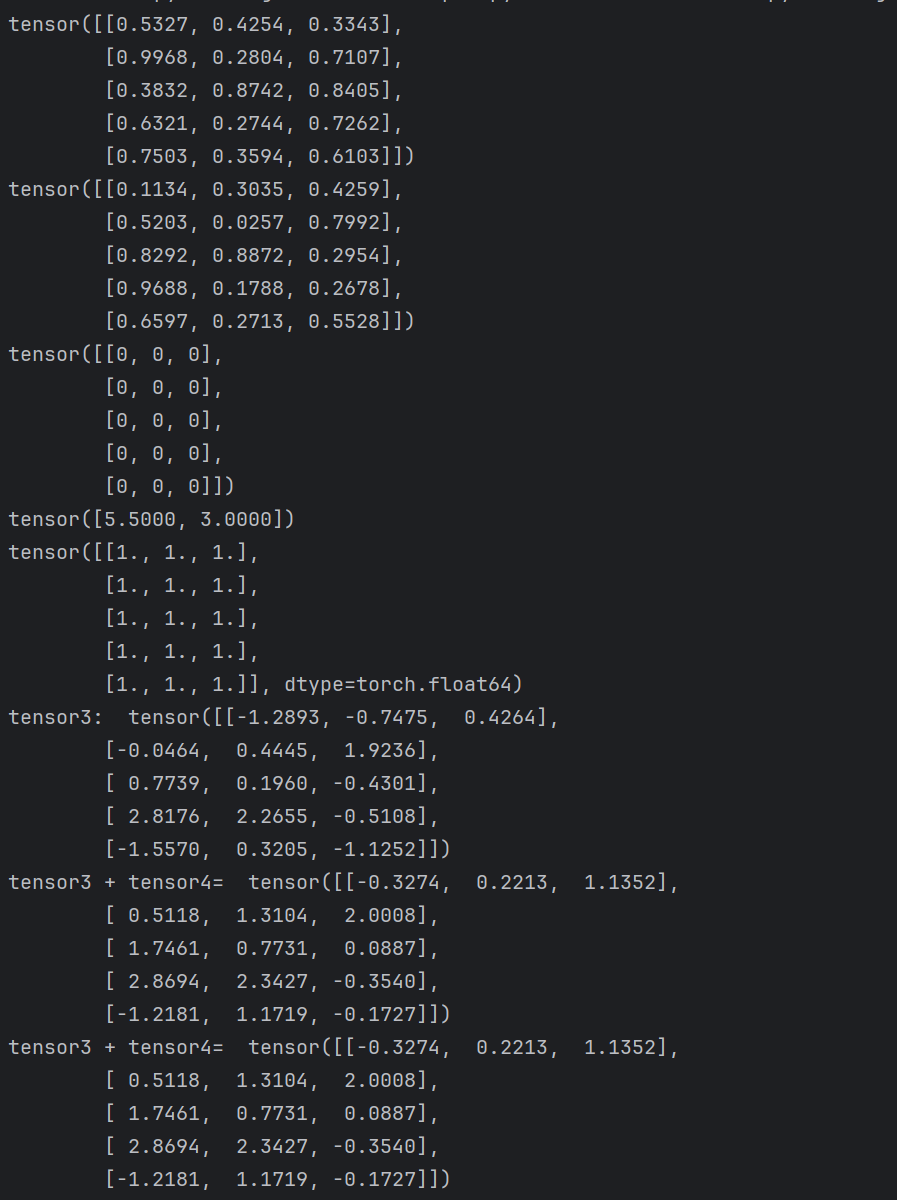
\includegraphics[width=0.8\textwidth]{6.png}
\caption{运行结果}
\end{figure}

\begin{figure}[htbp]
\centering
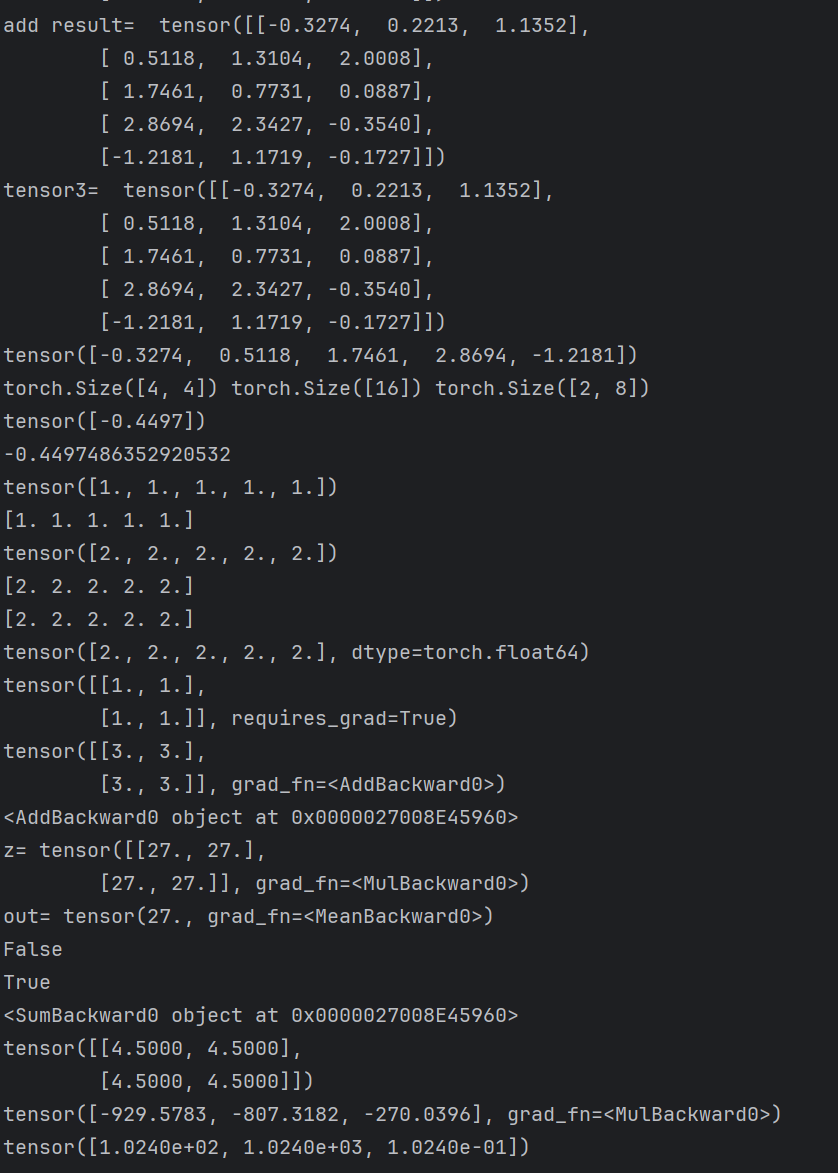
\includegraphics[width=0.8\textwidth]{7.png}
\caption{运行结果}
\end{figure}

\begin{figure}[htbp]
\centering
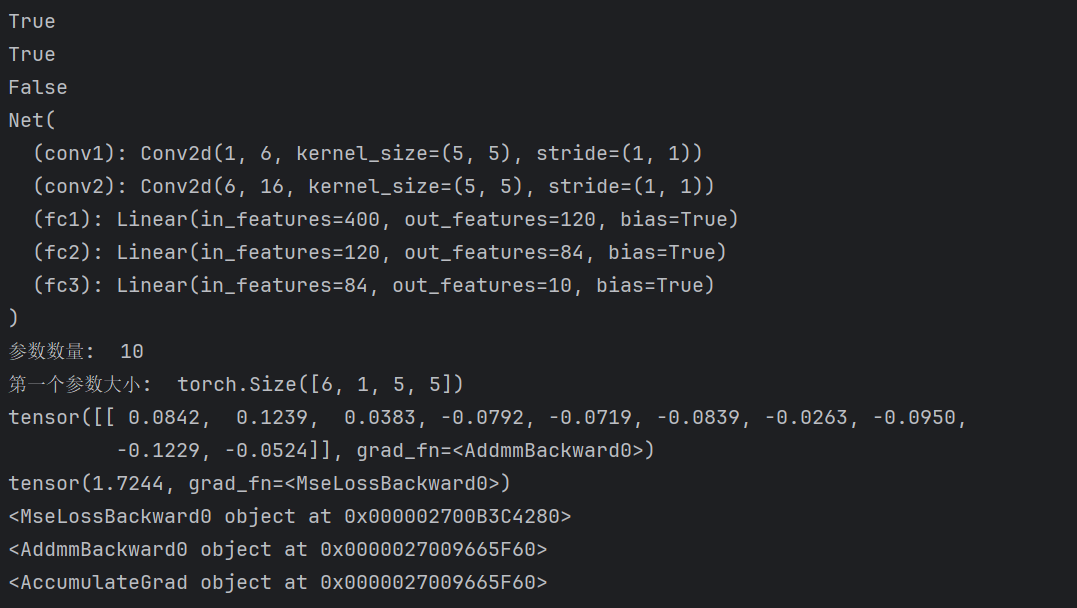
\includegraphics[width=0.8\textwidth]{8.png}
\caption{运行结果}
\end{figure}
\newpage
\section{心得体会}
学习调试、元编程、工具使用以及PyTorch的过程中,我深刻体会到这些技术不仅仅是工具的掌握,更是对编程思维的提升。最初接触调试时,我认为它只是找出程序错误的手段,但随着深入使用gdb等工具,我逐渐理解到,调试是为了保证程序的健壮性与效率。性能分析工具可以帮助我发现代码中的瓶颈,优化内存和资源的使用,从而提升整体运行效率。这让我意识到,代码不仅要完成功能,还要关注长远的性能和资源消耗。
元编程则为我带来了编程思维上的突破。通过学习模板和宏等技术,我开始理解编写通用、可复用代码的重要性。元编程不仅减少了重复劳动,更让我从更高层次上看待系统设计。这种编程方式鼓励我跳出具体问题,从抽象层面思考如何通过生成代码来提升开发效率。
工具的合理使用极大地提升了我的工作效率。通过自动化脚本和命令行优化,我将许多重复性任务自动化,大大节省了时间,同时提高了生产力。
在学习PyTorch的过程中,我对深度学习有了更深的理解。PyTorch灵活的动态计算图结构让我可以随时调试、修改模型,尤其适合快速实验和复杂模型的研究。其GPU加速和自动求导功能帮助我快速实现复杂的神经网络训练,缩短了从理论到实际应用的路径。

\section{github链接}
https://github.com/wj866/ouc.git
\end{document}